\section{Beispielrechnungen}
Wie lassen sich diese Kenntnisse nun nutzen, um den \ce{CO2}-Gehalt zu bestimmen?

\subsection*{Beispiel 1:}
\textbf{Berechnung des \ce{CO2}-Gehaltes für eine bestimmte Personenzahl zu einem bestimmten Zeitpunkt t}\\

\textit{10 Studenten sind in einem Seminarraum $\left(V = \SI{150}{\kmeter}\right)$ mit gekippten Fenstern $\left(n = \SI{0,3}{\per \hour}\right)$ und es soll der \ce{CO2}-Gehalt nach \SI{1,5}{\hour} bestimmt werden. Da alle Personen sitzende Tätigkeiten ausführen kann von einer spezifischen Emissionsrate von \SI{17}{\liter\per\hour} an \ce{CO2} ausgegangen werden.}\\

\begin{minipage}[t]{0.45\textwidth}
	\textbf{Gegeben:}
	\begin{itemize}
		\item Personenzahl $N = 10$
		\item Luftwechselzahl $n = \SI{0,3}{\per \hour}$
		\item Raumvolumen $n = \SI{150}{\kmeter}$
		\item Zeit $t = \SI{1,5}{\hour}$
	\end{itemize}
\end{minipage}
\begin{minipage}[t]{0.5\textwidth}
	\textbf{}
	\begin{itemize}
		\item spezifische Emissionsrate $\dot{V}_{\ce{CO2}} = \SI{17}{\liter \per \hour} = \SI{17e-3}{\kmeter \per \hour}  $
		\item Außenkonzentration \ce{CO2} \\
		$c_{\ce{CO2}, \text{außen}} = \SI{4}{\volpercent}$
	\end{itemize}
\end{minipage}
\FloatBarrier

\vspace*{5mm}

\begin{minipage}[t]{0.7\textwidth}
	\textbf{Gesucht:}
	\begin{itemize}
		\item \ce{CO2}-Gehalt zum Zeitpunkt t
	\end{itemize}
\end{minipage}

\vspace*{5mm}

\textbf{Skizze:}
\begin{figure}[h!]
	\centering
	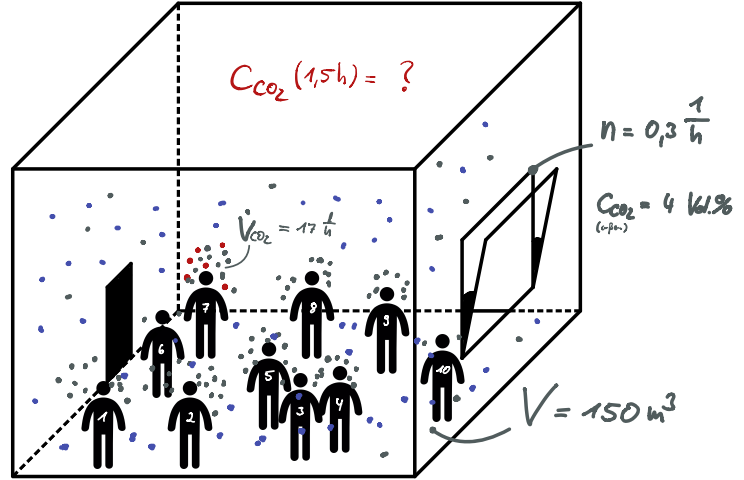
\includegraphics[width=0.5\textwidth]{img/beispiel 1}
	\caption{Skizze zu Beispiel 1}
	\label{fig:beispiel1}
\end{figure}
\FloatBarrier
%Ende

\newpage

\textbf{Lösung}:

\begin{flalign}
		\label{gl:beispiel1}
		c_{\ce{CO2}} (t) &= c_{\ce{CO2}, \text{außen}} + \frac{N*\dot{V}_{\ce{CO2}}}{10*n*V}*\left[1-e^{-n*t}\right]\\
		c_{\ce{CO2}} (\SI{1,5}{\hour}) &= \SI{0,04}{\volpercent} + \frac{10*\SI{17}{\liter\per \hour}}{10*\SI{0,3}{\per \hour}*\SI{150}{\kmeter}}*\left[1-e^{-\SI{0,3}{\per \hour}*\SI{1,5}{\hour}}\right]\\
						&= \SI{0,04}{\volpercent} +  \SI{0,137}{\volpercent}\\
						&= \underline{\SI{0,177}{\volpercent}}
\end{flalign}
\textit{Grenzkonzentration für DIN 1946 Teil II und \textsc{Pettenkofer}-Zahl überschritten!}

\subsection*{Beispiel 2:}
\textbf{Iterative Berechnung der Zeit t bis Grenzkonzentration erreicht ist}\\

\textit{Sieben Personen treffen sich zum studentischen Gelage in einer WG am Campus mit \SI{145}{\kmeter} Raumvolumen. Da ein halbgeöffnetes Fenster existiert, wird eine Luftwechselzahl von $n = \SI{0,26}{\per \hour}$ und durch den Milchgenuss eine Emissionsrate von \SI{25}{\liter \per \hour} gemessen. Die Außenkonzentration bleibt bei \SI{0,04}{\volpercent}. Es ist die Zeit zu bestimmen nach welcher eine Grenzkonzentration von \SI{0,15}{\volpercent} erreicht ist.}
\vspace*{5mm}

\begin{minipage}[t]{0.45\textwidth}
	\textbf{Gegeben:}
	\begin{itemize}
		\item Personenzahl $N = 7$
		\item Luftwechselzahl $n = \SI{1,05}{\per \hour}$
		\item Raumvolumen $n = \SI{145}{\kmeter}$
		\item Grenzkonzentration $c_{\ce{CO2}} = \SI{0,15}{\volpercent}$
	\end{itemize}
\end{minipage}
\begin{minipage}[t]{0.5\textwidth}
	\textbf{}
	\begin{itemize}
		\item spezifische Emissionsrate $\dot{V}_{\ce{CO2}} = \SI{25}{\liter \per \hour} $
		\item Außenkonzentration \ce{CO2} \\
		$c_{\ce{CO2}, \text{außen}} = \SI{4}{\volpercent}$
	\end{itemize}
\end{minipage}
\FloatBarrier

\vspace*{5mm}

\begin{minipage}[t]{1.0\textwidth}
	\textbf{Gesucht:}
	\begin{itemize}
		\item Zeitpunkt $t$ bis Grenzkonzentration erreicht ist
	\end{itemize}
\end{minipage}

\newpage

\textbf{Was ist iteratives Rechnen ?}\\
Iterationsverfahren beschreiben eine schrittweise Annäherung an eine Lösung durch wiederholte Ausführung einer Rechenvorschrift. Die Anzahl der Wiederholungen ist dabei abhängig von einer Abbruchbedingung, wie zum Beispiel die Genauigkeit der Nachkommastellen des Ergebnisses.\\
Sinnvoll ist diese Art Berechnung wenn nicht genügend Informationen über Parameter vorliegen oder sich ein umstellen der Gleichung nach einem bestimmten Parameter, als zu komplex erweist. \\
In der verfahrenstechnischen Praxis findet sich das iterative Rechnen im Excel-Add-In \textit{Solver} wieder. Auch dieses Add-In rechnet mit der iterativen Methodik.

%\vspace{-5mm}
\begin{center}
	\begin{figure}[h!]
		\centering
		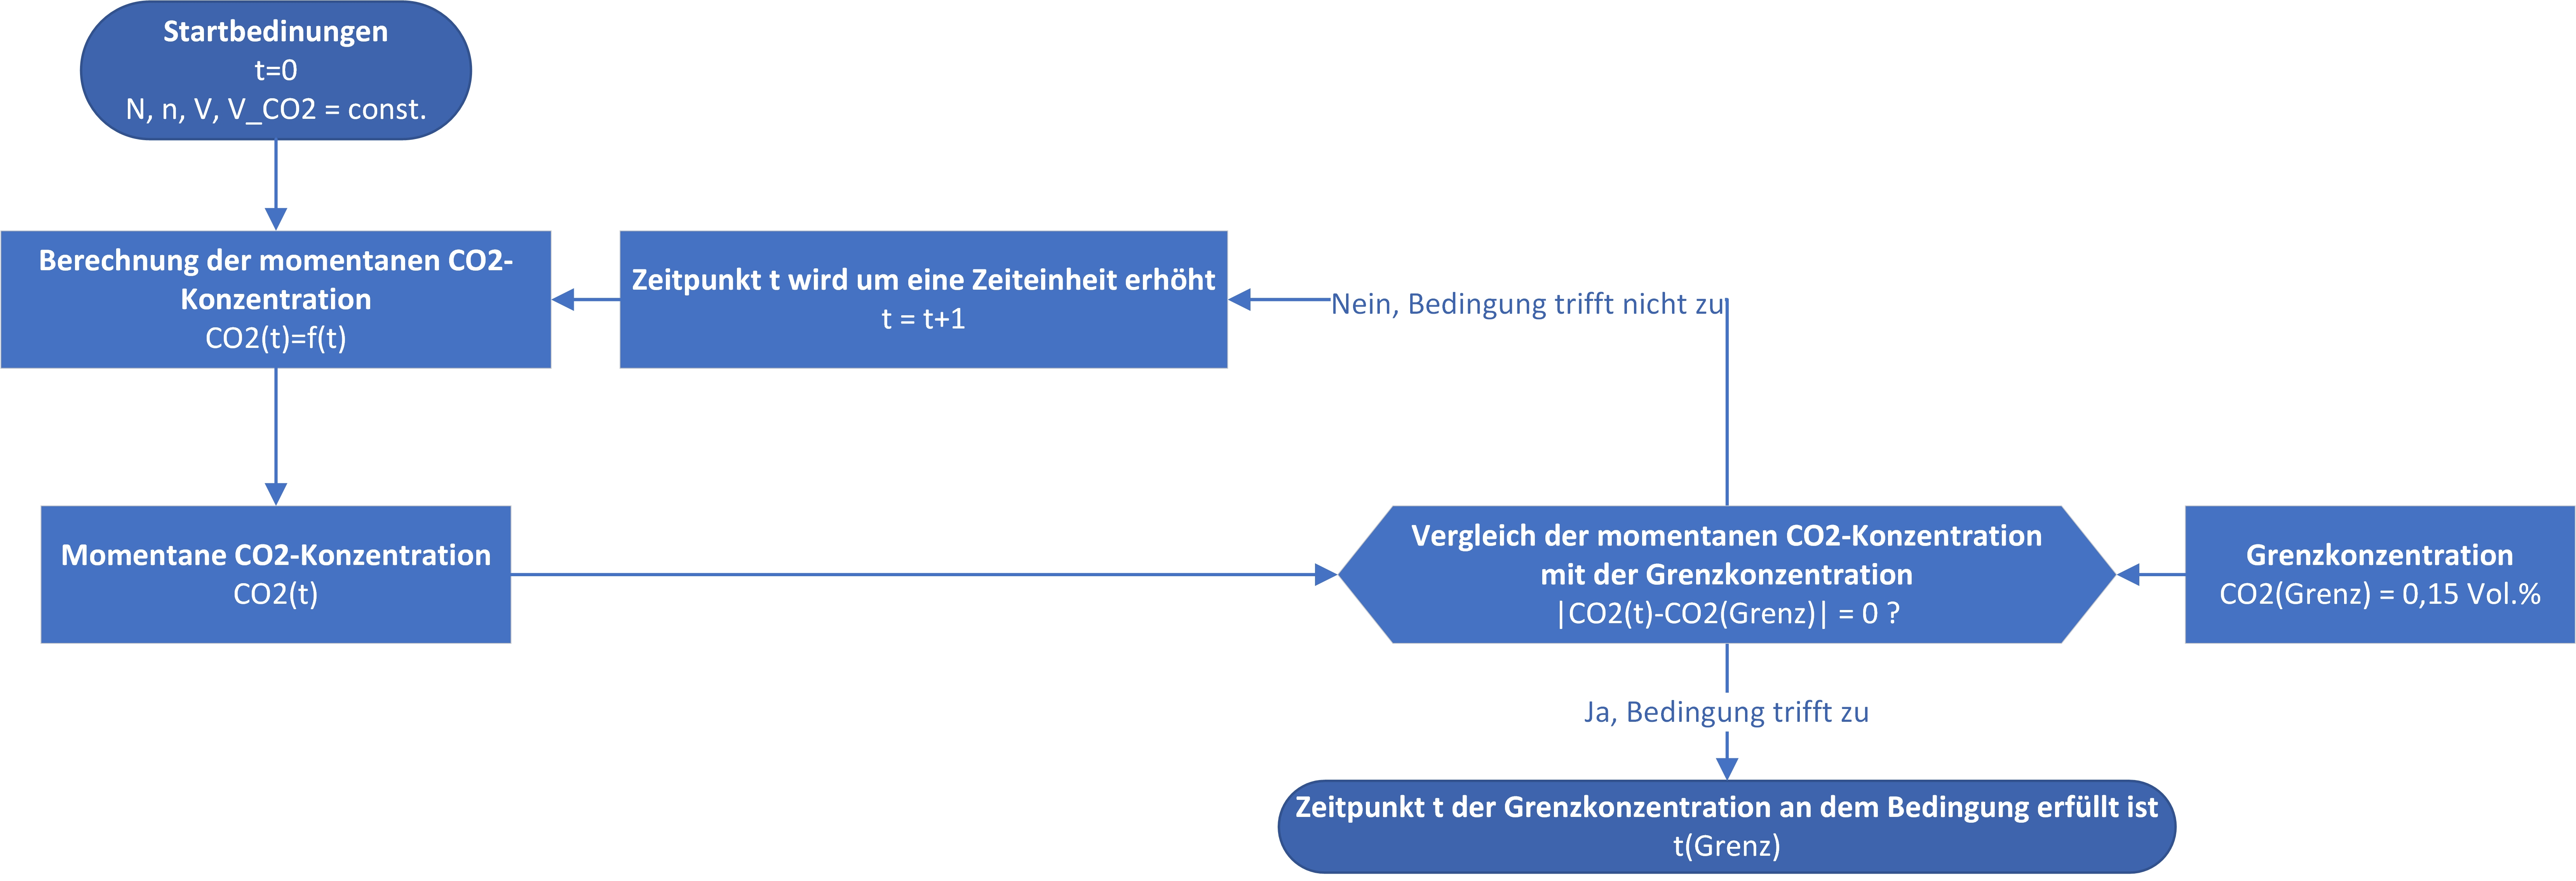
\includegraphics[width=1.1\textwidth]{img/iterativ}
		\caption{Übersicht zum iterativen Rechnen der \ce{CO2}-Konzentration}
\end{figure}
\end{center}

\FloatBarrier
%Ende

\newpage

\textbf{Lösung:}
\begin{enumerate}
	\item \textbf{Durchlauf} für $t = \SI{0}{\hour}$:\\
	\begin{flalign}
		c_{\ce{CO2}} (\SI{0}{\hour}) &= \SI{0,04}{\volpercent} + \frac{10*\SI{25}{\liter\per \hour}}{10*\SI{1,05}{\per \hour}*\SI{145}{\kmeter}}*\left[1-e^{-\SI{1,05}{\per \hour}*\SI{0}{\hour}}\right]\\
		&= \SI{0,040}{\volpercent}\\
		\Delta c_{\ce{CO2}} &= \abs{c_{\ce{CO2}}-c_{\text{Grenz}}}\\
													&=\abs{\SI{0,040}{\volpercent}-\SI{0,150}{\volpercent}}\\
													&= \SI{0,110}{\volpercent} > 0 \rightarrow \text{Wiederholung mit } t+1
	\end{flalign}
\item \textbf{Durchlauf} für $t = \SI{1}{\hour}$:\\
\begin{flalign}
	c_{\ce{CO2}} (\SI{1}{\hour}) &= \SI{0,04}{\volpercent} + \frac{10*\SI{25}{\liter\per \hour}}{10*\SI{1,05}{\per \hour}*\SI{145}{\kmeter}}*\left[1-e^{-\SI{1,05}{\per \hour}*\SI{1}{\hour}}\right]\\
	&= \SI{0,115}{\volpercent}\\
	\Delta c_{\ce{CO2}} &= \abs{\SI{0,115}{\volpercent}-\SI{0,150}{\volpercent}}\\
	&= \SI{0,035}{\volpercent} > 0 \rightarrow \text{Wiederholung mit } t+1
\end{flalign}
\item \textbf{Durchlauf} für $t = \SI{2}{\hour}$:\\
\begin{flalign}
	c_{\ce{CO2}} (\SI{2}{\hour}) &= \SI{0,04}{\volpercent} + \frac{10*\SI{25}{\liter\per \hour}}{10*\SI{1,05}{\per \hour}*\SI{145}{\kmeter}}*\left[1-e^{-\SI{1,05}{\per \hour}*\SI{2}{\hour}}\right]\\
	&= \SI{0,141}{\volpercent}\\
	\Delta c_{\ce{CO2}} &= \abs{\SI{0,141}{\volpercent}-\SI{0,150}{\volpercent}}\\
	&= \SI{0,009}{\volpercent} > 0 \rightarrow \text{Wiederholung mit } t+1
\end{flalign}
\item \textbf{Durchlauf} für $t = \SI{3}{\hour}$:\\
\begin{flalign}
	c_{\ce{CO2}} (\SI{3}{\hour}) &= \SI{0,04}{\volpercent} + \frac{10*\SI{25}{\liter\per \hour}}{10*\SI{1,05}{\per \hour}*\SI{145}{\kmeter}}*\left[1-e^{-\SI{1,05}{\per \hour}*\SI{3}{\hour}}\right]\\
	&= \SI{0,150}{\volpercent}\\
	\Delta c_{\ce{CO2}} &= \abs{\SI{0,150}{\volpercent}-\SI{0,150}{\volpercent}}\\
	&= \SI{0,000}{\volpercent} = 0 \rightarrow \text{Zeit der Grenzkonzentration}
\end{flalign}
\end{enumerate}

\newpage

\subsection*{Beispiel 3:}
\textbf{Einfluss der Personenzahl auf den Verlauf der \ce{CO2}-Konzentration}\\

\textit{Es soll der Verlauf der Konzentration an \ce{CO2} in Abhängigkeit von einer, 10 und 20 Personen grafisch dargestellt werden. Der Raum hat ein Volumen von \SI{145}{\kmeter} und es ist von einer Luftwechselzahl von \SI{1,05}{\per \hour} auszugehen. Es wurde eine Außenkonzentration von \SI{0,04}{\volpercent}, sowie eine spezifischen Emissionsrate von \SI{25}{\liter\per\hour} an \ce{CO2}.}

% Table generated by Excel2LaTeX from sheet 'Tabelle1'
\begin{table}[h!]
	\renewcommand*{\arraystretch}{1.2}
	\centering
	\rowcolors{2}{white}{gray!25}
	\caption{Daten für \ce{CO2}-Konzentration für verschiedenen Personenzahlen}
	\resizebox{\textwidth}{!}{
	\begin{tabulary}{1.0\textwidth}{c|ccc|cc}
		\hline
		Zeit [h]&c [Vol.\%] für 1 Pers. & c [Vol.\%] für 10 Pers.& c [Vol.\%] für 20 Pers. & \textsc{Pettenkofer}-Zahl & DIN 1946 Teil 2 \\
		\hline
		0,00  & 0,040 & 0,040 & 0,040 & 0,10   & 0,15 \\
		0,25  & 0,059 & 0,078 & 0,116 & 0,10   & 0,15 \\
		0,50  & 0,074 & 0,107 & 0,174 & 0,10   & 0,15 \\
		0,75  & 0,085 & 0,129 & 0,219 & 0,10   & 0,15 \\
		1,00  & 0,093 & 0,147 & 0,253 & 0,10   & 0,15 \\
		1,25  & 0,100 & 0,160 & 0,280 & 0,10   & 0,15 \\
		1,50  & 0,105 & 0,170 & 0,300 & 0,10   & 0,15 \\
		1,75  & 0,109 & 0,178 & 0,316 & 0,10   & 0,15 \\
		2,00  & 0,112 & 0,184 & 0,328 & 0,10   & 0,15 \\
	\end{tabulary}%
	\label{tab:tabelle_co2}%
}
\end{table}%


\begin{figure}[h!]
	\begin{center}
		\resizebox{0.75\textwidth}{!}{
			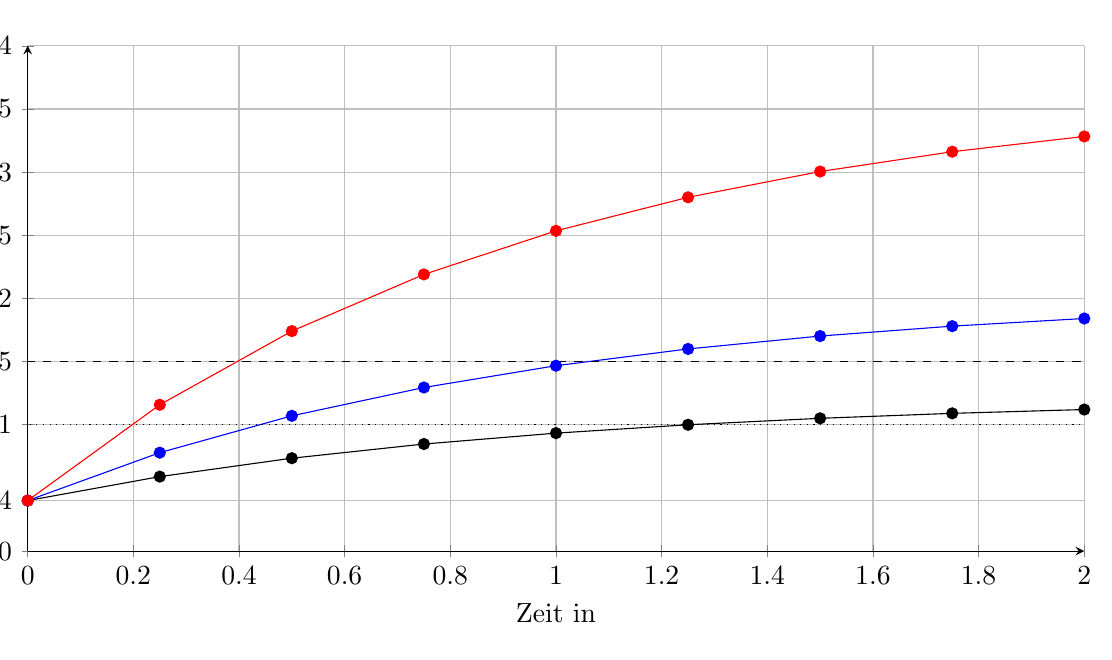
\begin{tikzpicture}[trim axis left, trim axis right]
				\begin{axis}[
					grid =both,
					axis lines = left,
					width = 15cm,
					height = 8cm,
					xmin = 0,
					xmax = 2.,
					ymin = 0,
					ymax = 0.4,
					ytick = {0,0.04,0.1,0.15,...,0.4},
					%xtick = {0,1,...,5},
					ylabel={\ce{CO2}-Konzentration in \si{\volpercent}},
					%y label style={at={(0,0.5)}},
					xlabel={Zeit in \si{\hour}},
					legend style={at={(1.05,0.75)},anchor=west},
					%	y dir = reverse,
					yticklabel style={/pgf/number format/fixed},
					]
					
					%1 Person
					\addplot [color=black, mark=*] coordinates{(0,0.04) (0.25,5.89551424984753E-02) (0.5,7.35340423344158E-02) (0.75,8.47470585617263E-02) (1,9.33712849662434E-02) (1.25,0.100004404866241) (1.5,0.105106112259347) (1.75,0.109029969918679) (2,0.112047912294501)};
					
					%10 Person
					\addplot [color=blue, mark=*] coordinates{(0,0.04) (0.25,7.79102849969507E-02) (0.5,0.107068084668832) (0.75,0.129494117123453) (1,0.146742569932487) (1.25,0.160008809732482) (1.5,0.170212224518694) (1.75,0.178059939837358) (2,0.184095824589001)};
					
					%20 Person
					\addplot [color=red, mark=*] coordinates{(0,0.04) (0.25,0.115820569993901) (0.5,0.174136169337663) (0.75,0.218988234246905) (1,0.253485139864974) (1.25,0.280017619464964) (1.5,0.300424449037388) (1.75,0.316119879674716) (2,0.328191649178003) };
					
					\addplot[mark=none, black, dotted, samples=2] {0.1};
					\addplot[mark=none, black, dashed, samples=2] {0.15};
				 
				 	\legend{1 Person, 10 Personen, 20 Personen, \textsc{Pettenkofer}-Zahl, DIN 1946 Teil 2}
				\end{axis}
			\end{tikzpicture}
		}
		\caption{Verlauf der gemittelten Temperaturdifferenzen}
		\label{dia:tdiffverlauf}
	\end{center}
\end{figure}
\FloatBarrier